\documentclass{article}
\usepackage{graphicx}
\usepackage{authblk}
\usepackage{amsmath}
\usepackage{listings}

\begin{document}


\title{THEORETICAL NEUROSCIENCE II \\ EXERCISE - OCULAR DOMINANCE}
\date{27 Mai. 2013}
\author[1]{Yunus Emre Demiray, Taygun C. Uzuneser, \c{S}eyma Bayrak\thanks{seyma.bayrak@st.ovgu.de}}
\affil[1]{\footnotesize  Otto von Guericke University of Magdeburg}
\maketitle

\newpage

\section{Input Correlations}
We consider the rates of two LGN afferents, $u_R$ from the right eye and $u_L$ from the left eye such that they are binary, either 1 or 0, and their average is 0.5. The first task is to generate different input pairs of ($u_R,u_L$). The joint probabilities are defined as the following by a limiting $\gamma$ value.

\begin{equation*}
u_{R,L} \;\; \epsilon \;\;\{0,1\} \;\;\;\;\;\;\ \langle u_R \rangle = \langle u_L \rangle = \frac{1}{2}
\end{equation*}
\begin{equation*}
  p_1=p_0=\frac{1}{2} \;\;\;\;\;\;\ p_{11}=p_{00}=\frac{\gamma}{4} \;\;\;\;\;\;\ p_{01}=p_{10}=\frac{1}{2}-\frac{\gamma}{4} \;\;\;\;\;\;\ 0\leq \gamma \leq 2 
\end{equation*}

\begin{itemize}
 \item Use these probabilities to derive the correlation and covariance matrices for chosen values of $\gamma$, both analytically and numerically.
\end{itemize}
\begin{equation*}
 c_S= \langle u_L u_L \rangle - \langle u_L \rangle^2 =\langle u_R u_R \rangle - \langle u_R \rangle^2=\sum_{u_{R,L} \; \epsilon\{0,1\}} p_R .u_R .u_R-(\frac{1}{2})^2 
\end{equation*}
\begin{equation*} 
= p_1u_1u_1 -\frac{1}{4}=\frac{1}{2}.1.1 -\frac{1}{4}=\frac{1}{2}-\frac{1}{4}=\frac{1}{4} \
\end{equation*}

\begin{equation*}
 c_D=\langle u_R u_L \rangle - \langle u_R \rangle . \langle u_L \rangle  =\sum_{u_{R,L} \; \epsilon\{0,1\}} p_{RL}.u_R.u_L-\frac{1}{2}.\frac{1}{2}
\end{equation*}
\begin{equation*}
 =p_{00}.0.0+p_{01}.0.1+p_{11}.1.1+p_{10}.1.0 -\frac{1}{4}=\frac{¸\gamma}{4}-\frac{1}{4}=\frac{1}{4}(\gamma-1)
\end{equation*}
The covariance matrix turns out to be the following:
\begin{equation}
\ C= \left ( \begin{array}{cc} c_S & c_D \\ c_D & c_S \end{array} \right ) \  =  \left ( \begin{array}{cc} \frac{1}{4} & \frac{1}{4}(\gamma-1) \\ \frac{1}{4}(\gamma-1) & \frac{1}{4} \end{array} \right ) \ 
\end{equation}

Now, let us calculate the coefficients for the correlation matrix.
\begin{equation*}
 q_S=\langle u_R^2 \rangle = \langle u_L^2 \rangle=\sum_{u_{R,L} \; \epsilon\{0,1\}} p_R .u_R.u_R=p_0.0.0+p_1.1.1=\frac{1}{2} 
\end{equation*}
\begin{equation*}
 q_D=\langle u_R u_L \rangle=\sum_{u_{R,L} \; \epsilon\{0,1\}} p_{RL} .u_R.u_L=\frac{\gamma}{4} 
\end{equation*}
The correlation matrix turns out to be the following:
\begin{equation}
\ Q= \left ( \begin{array}{cc} q_S & q_D \\ q_D & q_S \end{array} \right ) \  =  \left ( \begin{array}{cc} \frac{1}{2} & \frac{\gamma}{4} \\ \frac{\gamma}{4} & \frac{1}{2} \end{array} \right ) \ 
\end{equation}
The assignment asks for comparing the analytically calculated matrix in equation 1 with the numericlally calculated one. For a better understanding, the comparison is done 5 times with different $\gamma$ values such that $\gamma$=[0 0.25 0.5 0.75 1]. Both analytic and numerical solutions for covariance matrices for different $\gamma$ values are introduced below.

\begin{equation*}
 \gamma=0, \ C_{anly} =  \left ( \begin{array}{cc} 0.2500 & -0.2500 \\ -0.2500 & 0.2500 \end{array} \right ) \  \ C_{num} =  \left ( \begin{array}{cc} 0.2619 & -0.2499 \\ -0.2499 & 0.2619 \end{array} \right ) \
\end{equation*}

\begin{equation*}
 \gamma=0.25, \ C_{anly} =  \left ( \begin{array}{cc} 0.2500 & -0.1875 \\ -0.1875 & 0.2500 \end{array} \right ) \  \ C_{num} =  \left ( \begin{array}{cc} 0.2460 & -0.1910 \\ -0.1910 & 0.2460 \end{array} \right ) \
\end{equation*}

\begin{equation*}
 \gamma=0.5, \ C_{anly} =  \left ( \begin{array}{cc} 0.2500 & -0.1250 \\ -0.1250& 0.2500 \end{array} \right ) \  \ C_{num} =  \left ( \begin{array}{cc} 0.2358 & -0.1335 \\ -0.1335 & 0.2358 \end{array} \right ) \
\end{equation*}

\begin{equation*}
 \gamma=0.75, \ C_{anly} =  \left ( \begin{array}{cc} 0.2500 & -0.0625 \\ -0.0675 & 0.2500 \end{array} \right ) \  \ C_{num} =  \left ( \begin{array}{cc} 0.2510 & -0.0550 \\ -0.0550& 0.2510 \end{array} \right ) \
\end{equation*}

\begin{equation*}
 \gamma=1, \ C_{anly} =  \left ( \begin{array}{cc} 0.2500 & 0 \\ 0 & 0.2500 \end{array} \right ) \  \ C_{num} =  \left ( \begin{array}{cc} 0.2399 & 0 \\ 0 & 0.2399 \end{array} \right ) \
\end{equation*}

The provided MATLAB function \textbf{ShowEigen.m} plots the eigenvectors and eigenvalues for the numerically calculated \textbf{C} matrices for the different $\gamma$ values as the following.

\begin{center}
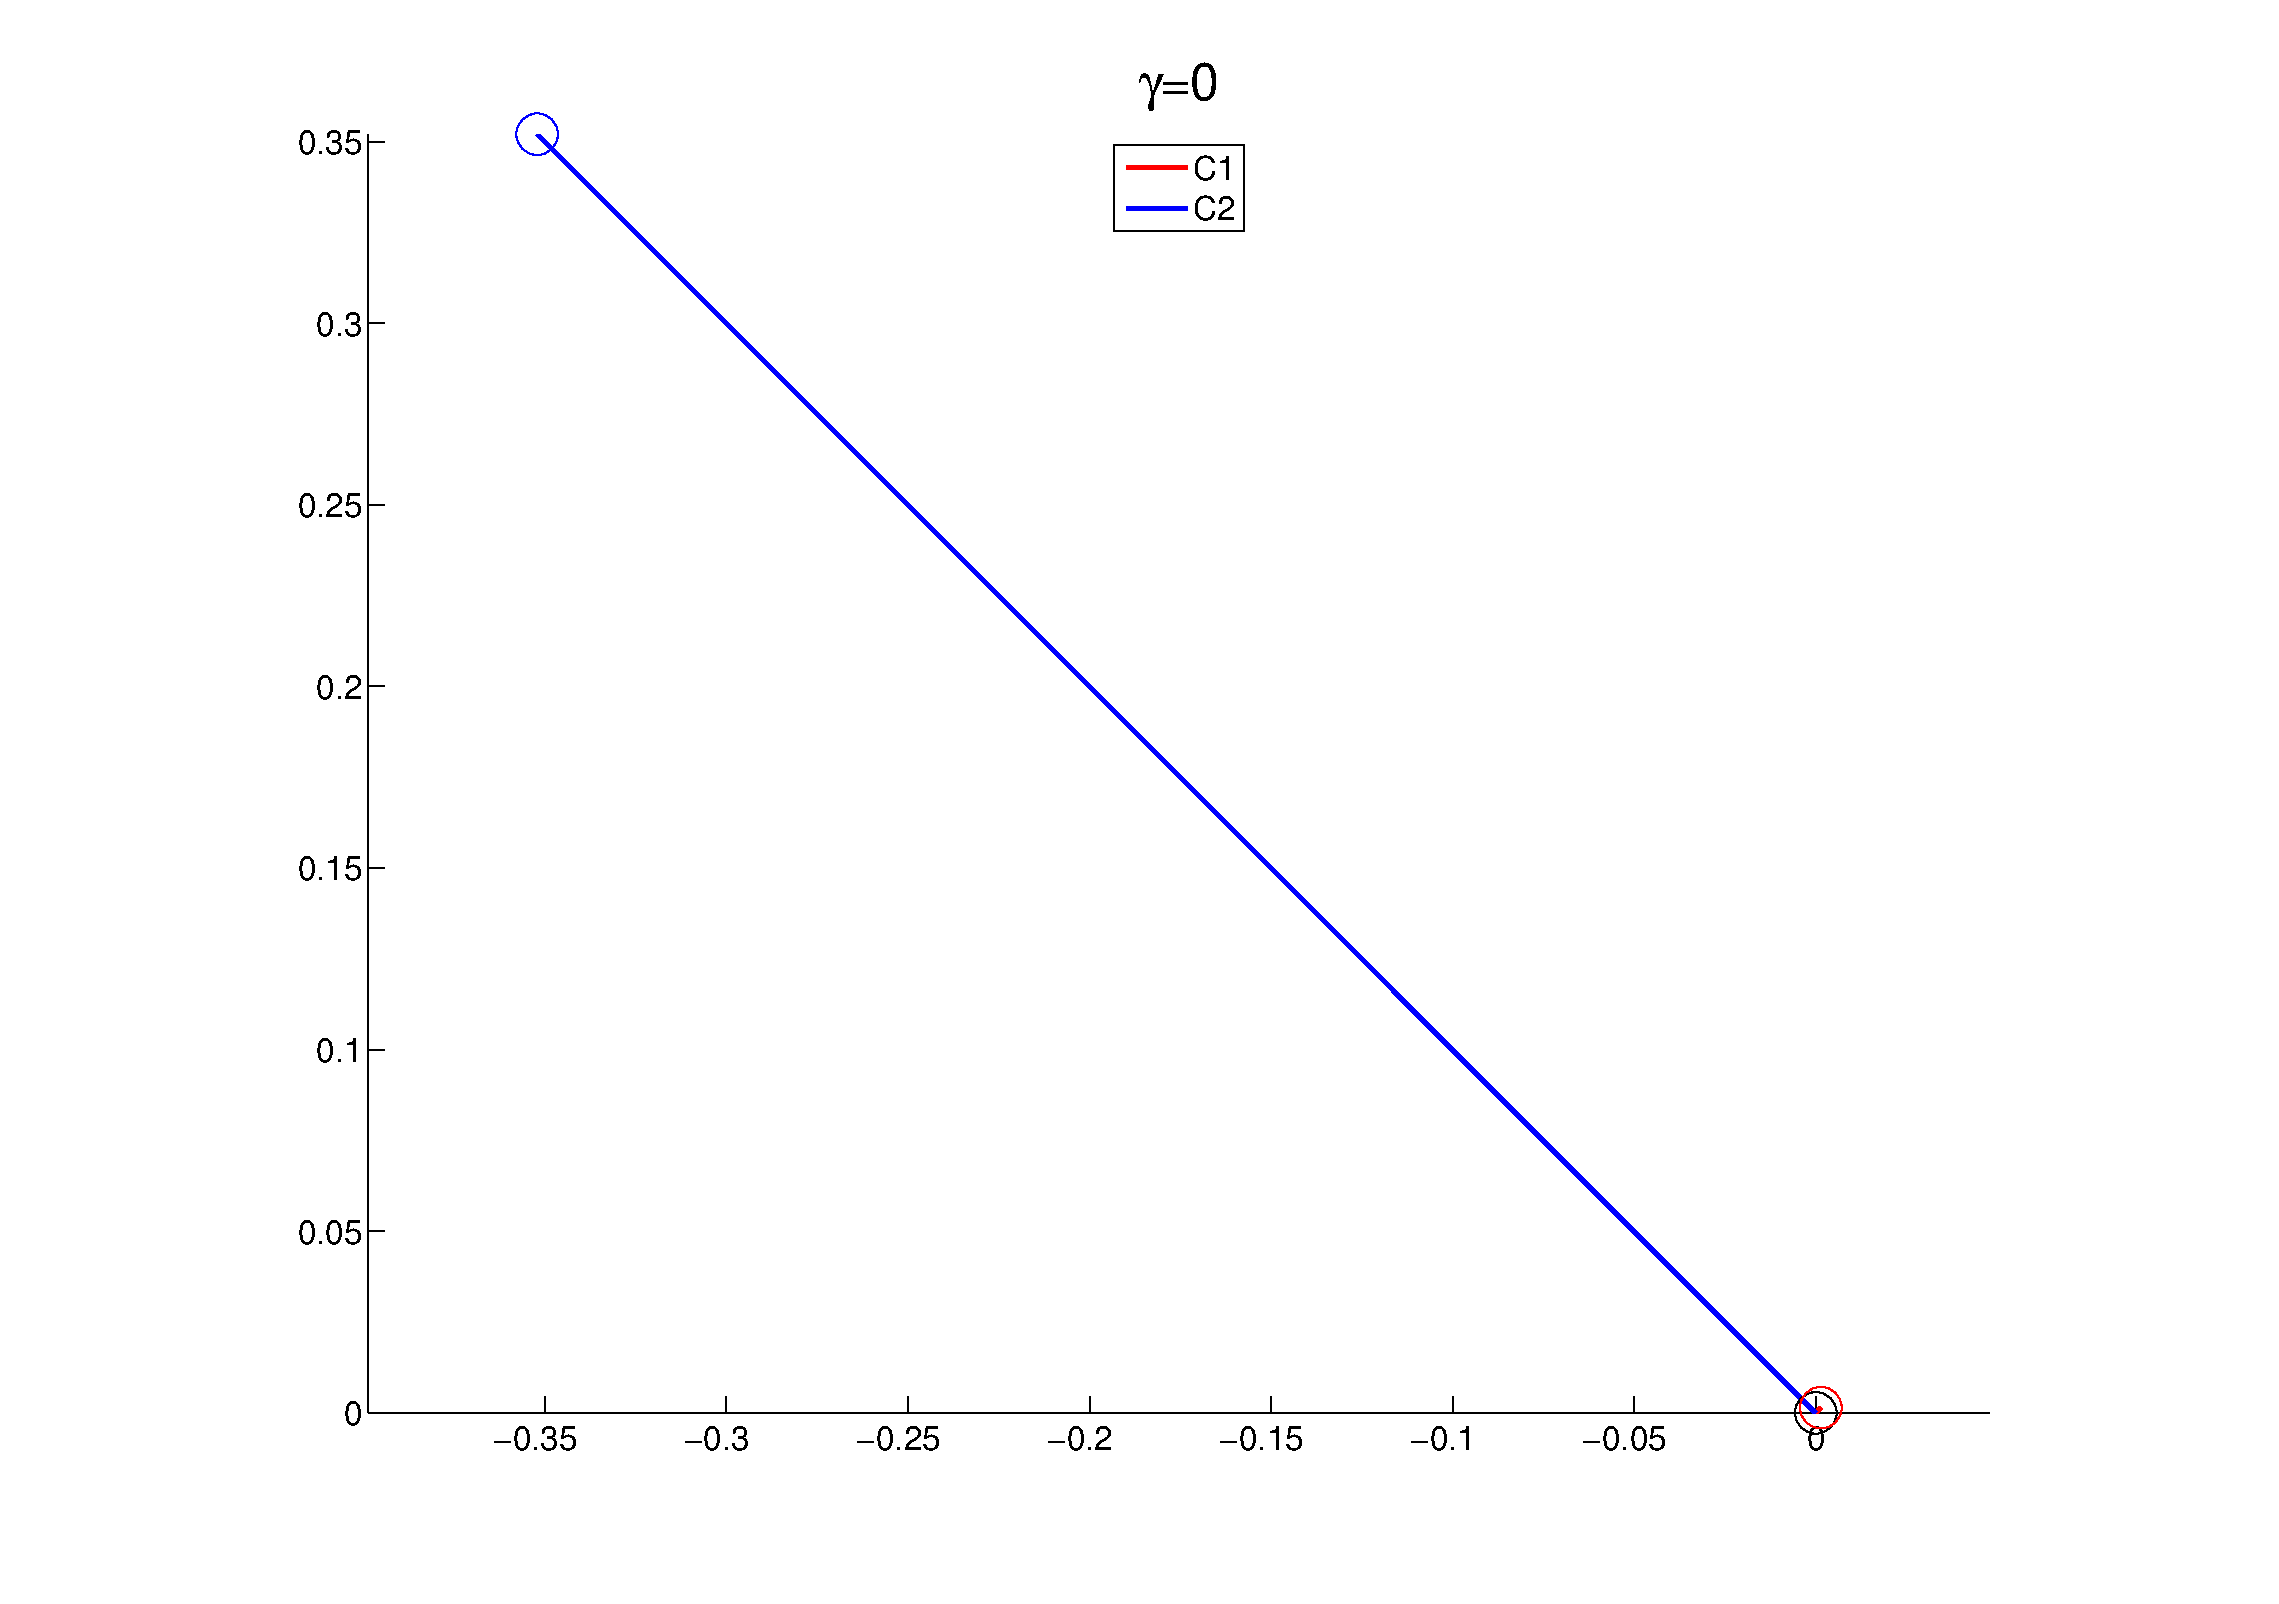
\includegraphics[width=\textwidth]{eigen1.eps}
% tau4_M1.eps: 0x0 pixel, 300dpi, 0.00x0.00 cm, bb= -304   -42   918   834
\begin{footnotesize}
 Figure 1, $\gamma=0$
\end{footnotesize}
\end{center}

\begin{center}
\includegraphics[width=\textwidth]{eigen2.eps}
% tau4_M1.eps: 0x0 pixel, 300dpi, 0.00x0.00 cm, bb= -304   -42   918   834
\begin{footnotesize}
 Figure 2, $\gamma=0.25$
\end{footnotesize}
\end{center}

\begin{center}
\includegraphics[width=\textwidth]{eigen3.eps}
% tau4_M1.eps: 0x0 pixel, 300dpi, 0.00x0.00 cm, bb= -304   -42   918   834
\begin{footnotesize}
 Figure 3, $\gamma=0.5$
\end{footnotesize}
\end{center}

\begin{center}
\includegraphics[width=\textwidth]{eigen4.eps}
% tau4_M1.eps: 0x0 pixel, 300dpi, 0.00x0.00 cm, bb= -304   -42   918   834
\begin{footnotesize}
 Figure 4, $\gamma=0.75$
\end{footnotesize}
\end{center}

\begin{center}
\includegraphics[width=\textwidth]{eigen5.eps}
% tau4_M1.eps: 0x0 pixel, 300dpi, 0.00x0.00 cm, bb= -304   -42   918   834
\begin{footnotesize}
 Figure 5, $\gamma=1$
\end{footnotesize}
\end{center}

\subsection{Discussion}
\begin{itemize}
 \item $\gamma$ value is assumed to give the probability of getting the same input from both eyes as $p_{00}=p_{11}=\gamma$. That means, if $\gamma$ increases, the probability of getting same inputs from both eyes must increase, so it means more binocularity. In other words, if the $\gamma$ value is defined to be small enough, the probability of getting different inputs from both eyes increase, this causes more monocularity. 

\item $\gamma$ decides if the covariance values are positive or negative. Additionally it decides how big or small the $c_D$ value is, since $c_D=0.25(1-\gamma)$, it has no effect on $c_S$. The numerically and anayltically builded covariance matrices seem to be reasonably well matching. It seems that we are on the right path.

\item Figures 1-5 show how the different $\gamma$ values change the covariance matrice \textbf{C}, and therefore its eigenvalues and eigenvectors. As the $\gamma$ increases, the two eigenvectors (blue and red lines) seem to be more distinctive. At small $\gamma$, one eigenvector dominates - called principal one -, at big $\gamma$ values they seem to dominate almost equally. In further parts of exercise this fact will be higlighted again. 
\end{itemize}



\section{One target neuron, no normalization}
We consider a single cell layer 4 of primary cortex (rate \textit{v}), which receives inputs from two LGN afferents $u_R,u_L$, one from the right eye, and the other from the right eye. The input weights $w_R,w_L$ change according to covariance rule, but restricted to the range $0\leq w_{R,L} \leq 1$:

\begin{equation}
 v=\textbf{u.w}=w_R u_R + w_L u_L
\end{equation}
\begin{equation}
 \tau_w=\frac{d\textbf{w}}{dt}=\textbf{Cw} \;\;\;\; where \;\;\;\; \ C= \left ( \begin{array}{cc} c_S & c_D \\ c_D & c_S \end{array} \right ) \  
\end{equation}

\begin{equation*}
 \tau_w=\frac{dw_R}{dt}=c_S w_R + c_D w_L \;\;\;\; and \;\;\;\; \tau_w=\frac{dw_L}{dt}=c_D w_R + c_S w_L
\end{equation*}

\begin{itemize}
 \item Iteratively compute trajectories for different starting points [$w_R(0),w_l(0)$] in the range of [0, 0.25], visualize the development in the space of connection states, spanned by $0\leq w_{R,L} \leq 1$. Use $\tau_m$=0.1 and $dt$=0.1. Dexcribe the different kinds of the development observed for different covariance matrices (different matrices is created by different $\gamma$ values).
\end{itemize}

The eigenvectors with the eigenvalues of 5 different covariance matrices are already plotted and shown in Figures 1-5. Now, the $w_R$ and $w_L$ are computed iteratively with those 5 covariance matrices and plotted below. \newpage

Let us choose the initial points fix but change the $\gamma$ values and observe the weights.
\begin{center}
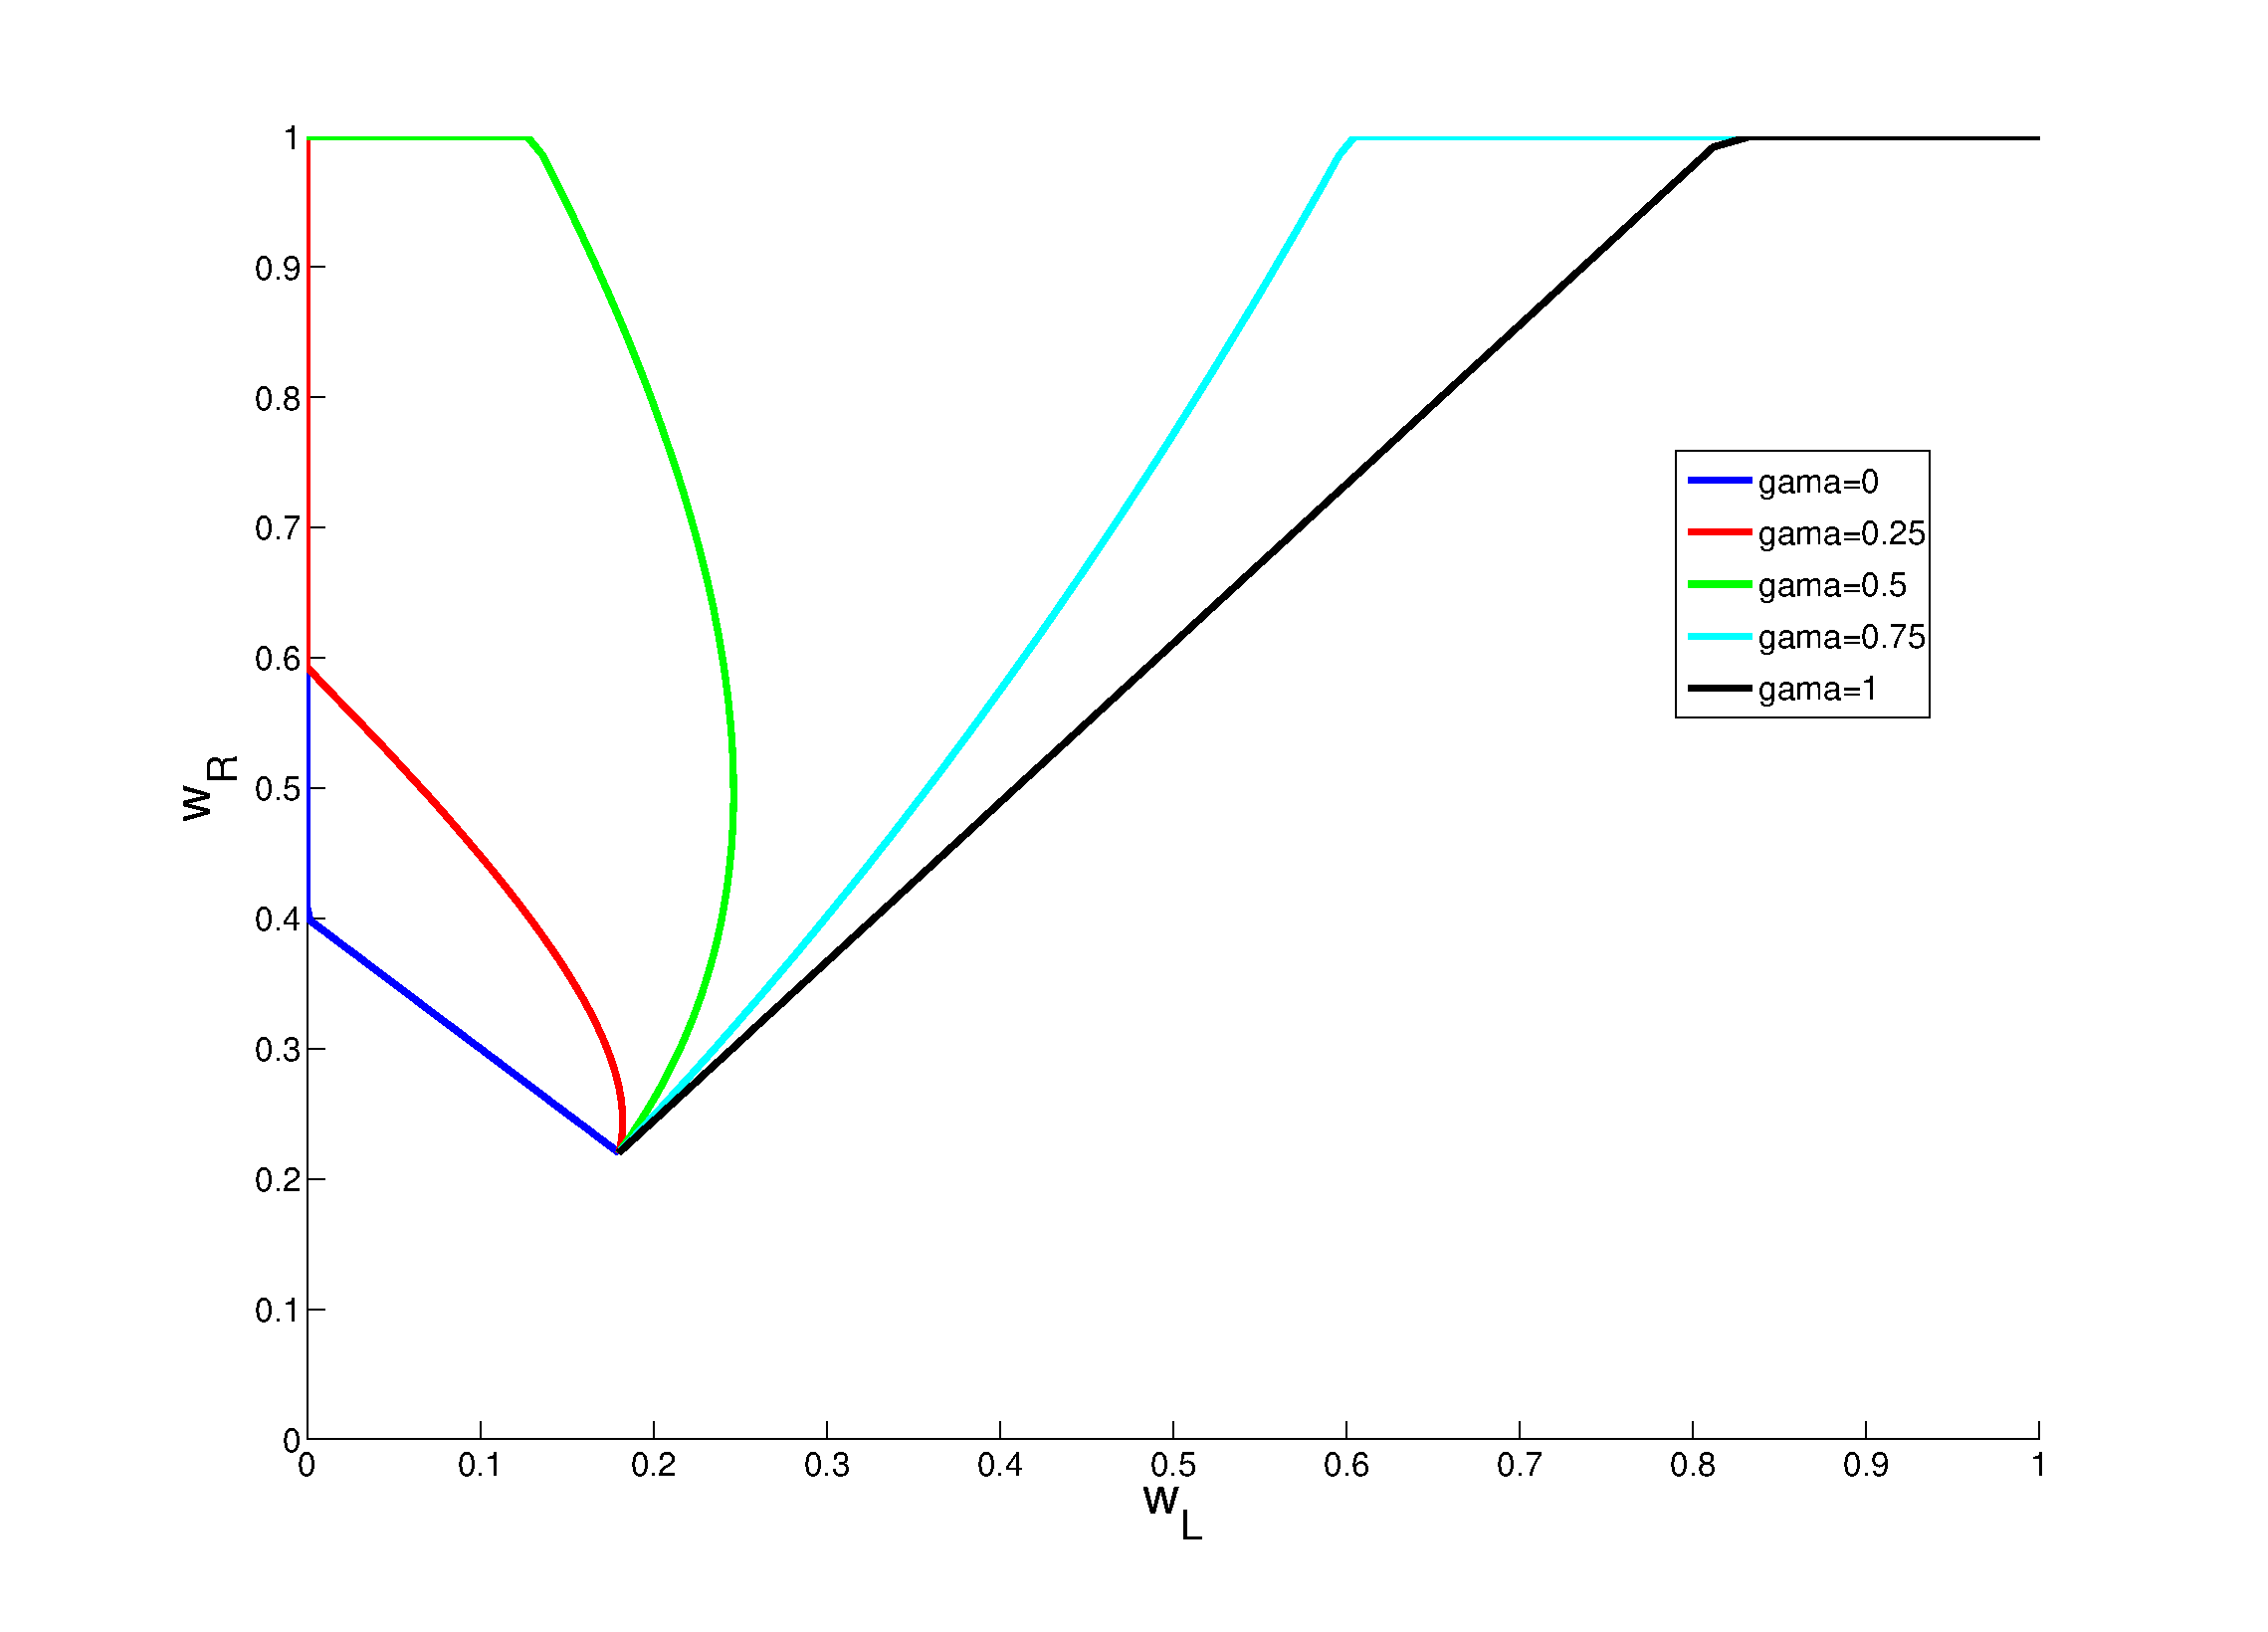
\includegraphics[width=\textwidth, height=75mm]{dif_gama.eps}
% tau4_M1.eps: 0x0 pixel, 300dpi, 0.00x0.00 cm, bb= -304   -42   918   834
\begin{footnotesize}
 Figure 6, initial points $w_R$=0.22, $w_L$=0.18, $\gamma$ values change between 0 and 1.
\end{footnotesize}
\end{center}

Let us choose one fixed $\gamma$ value, e.g. $\gamma=0.5$, do the same iteration shown in Equation 4 by different initial values to observe the effect of initial points on weights.

\begin{center}
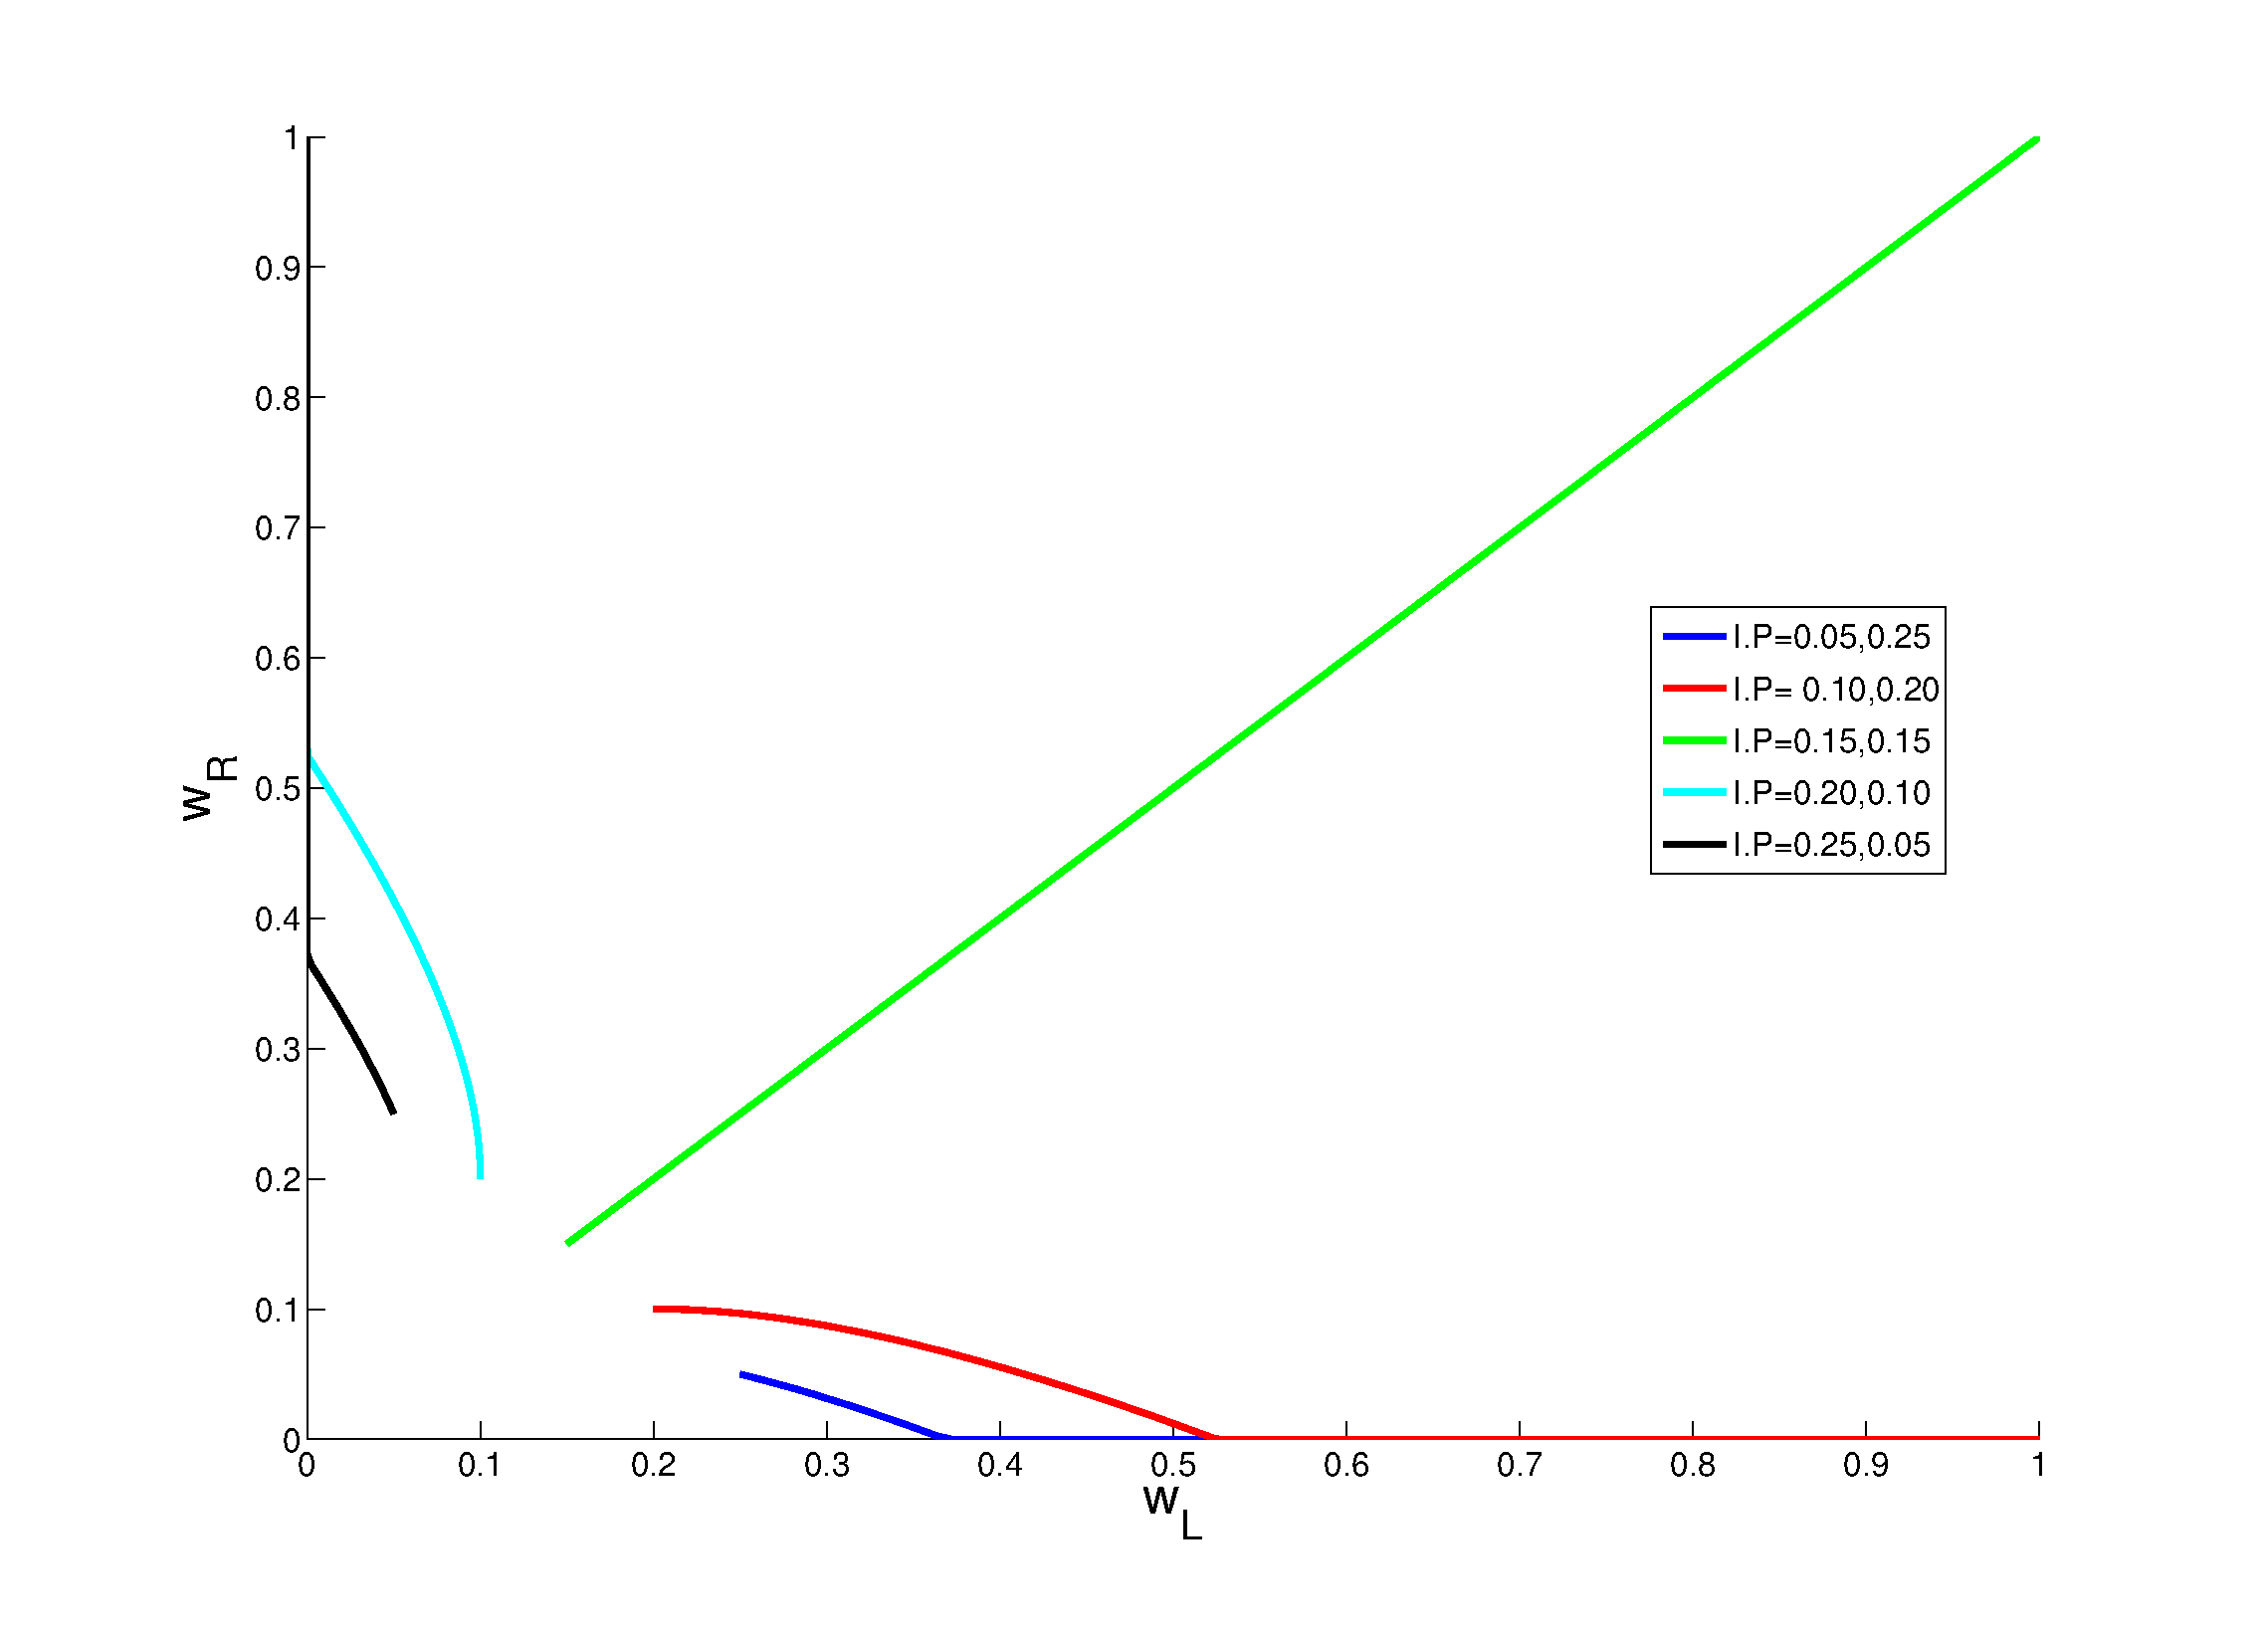
\includegraphics[width=\textwidth,  height=75mm]{5_initial.eps}
% tau4_M1.eps: 0x0 pixel, 300dpi, 0.00x0.00 cm, bb= -304   -42   918   834
\begin{footnotesize}
 Figure 7, $\gamma=0.5$, \textbf{I.P} legends on the graph refers to different initial points
\end{footnotesize}
\end{center}

What happens if more initial values are chosen?

\begin{center}
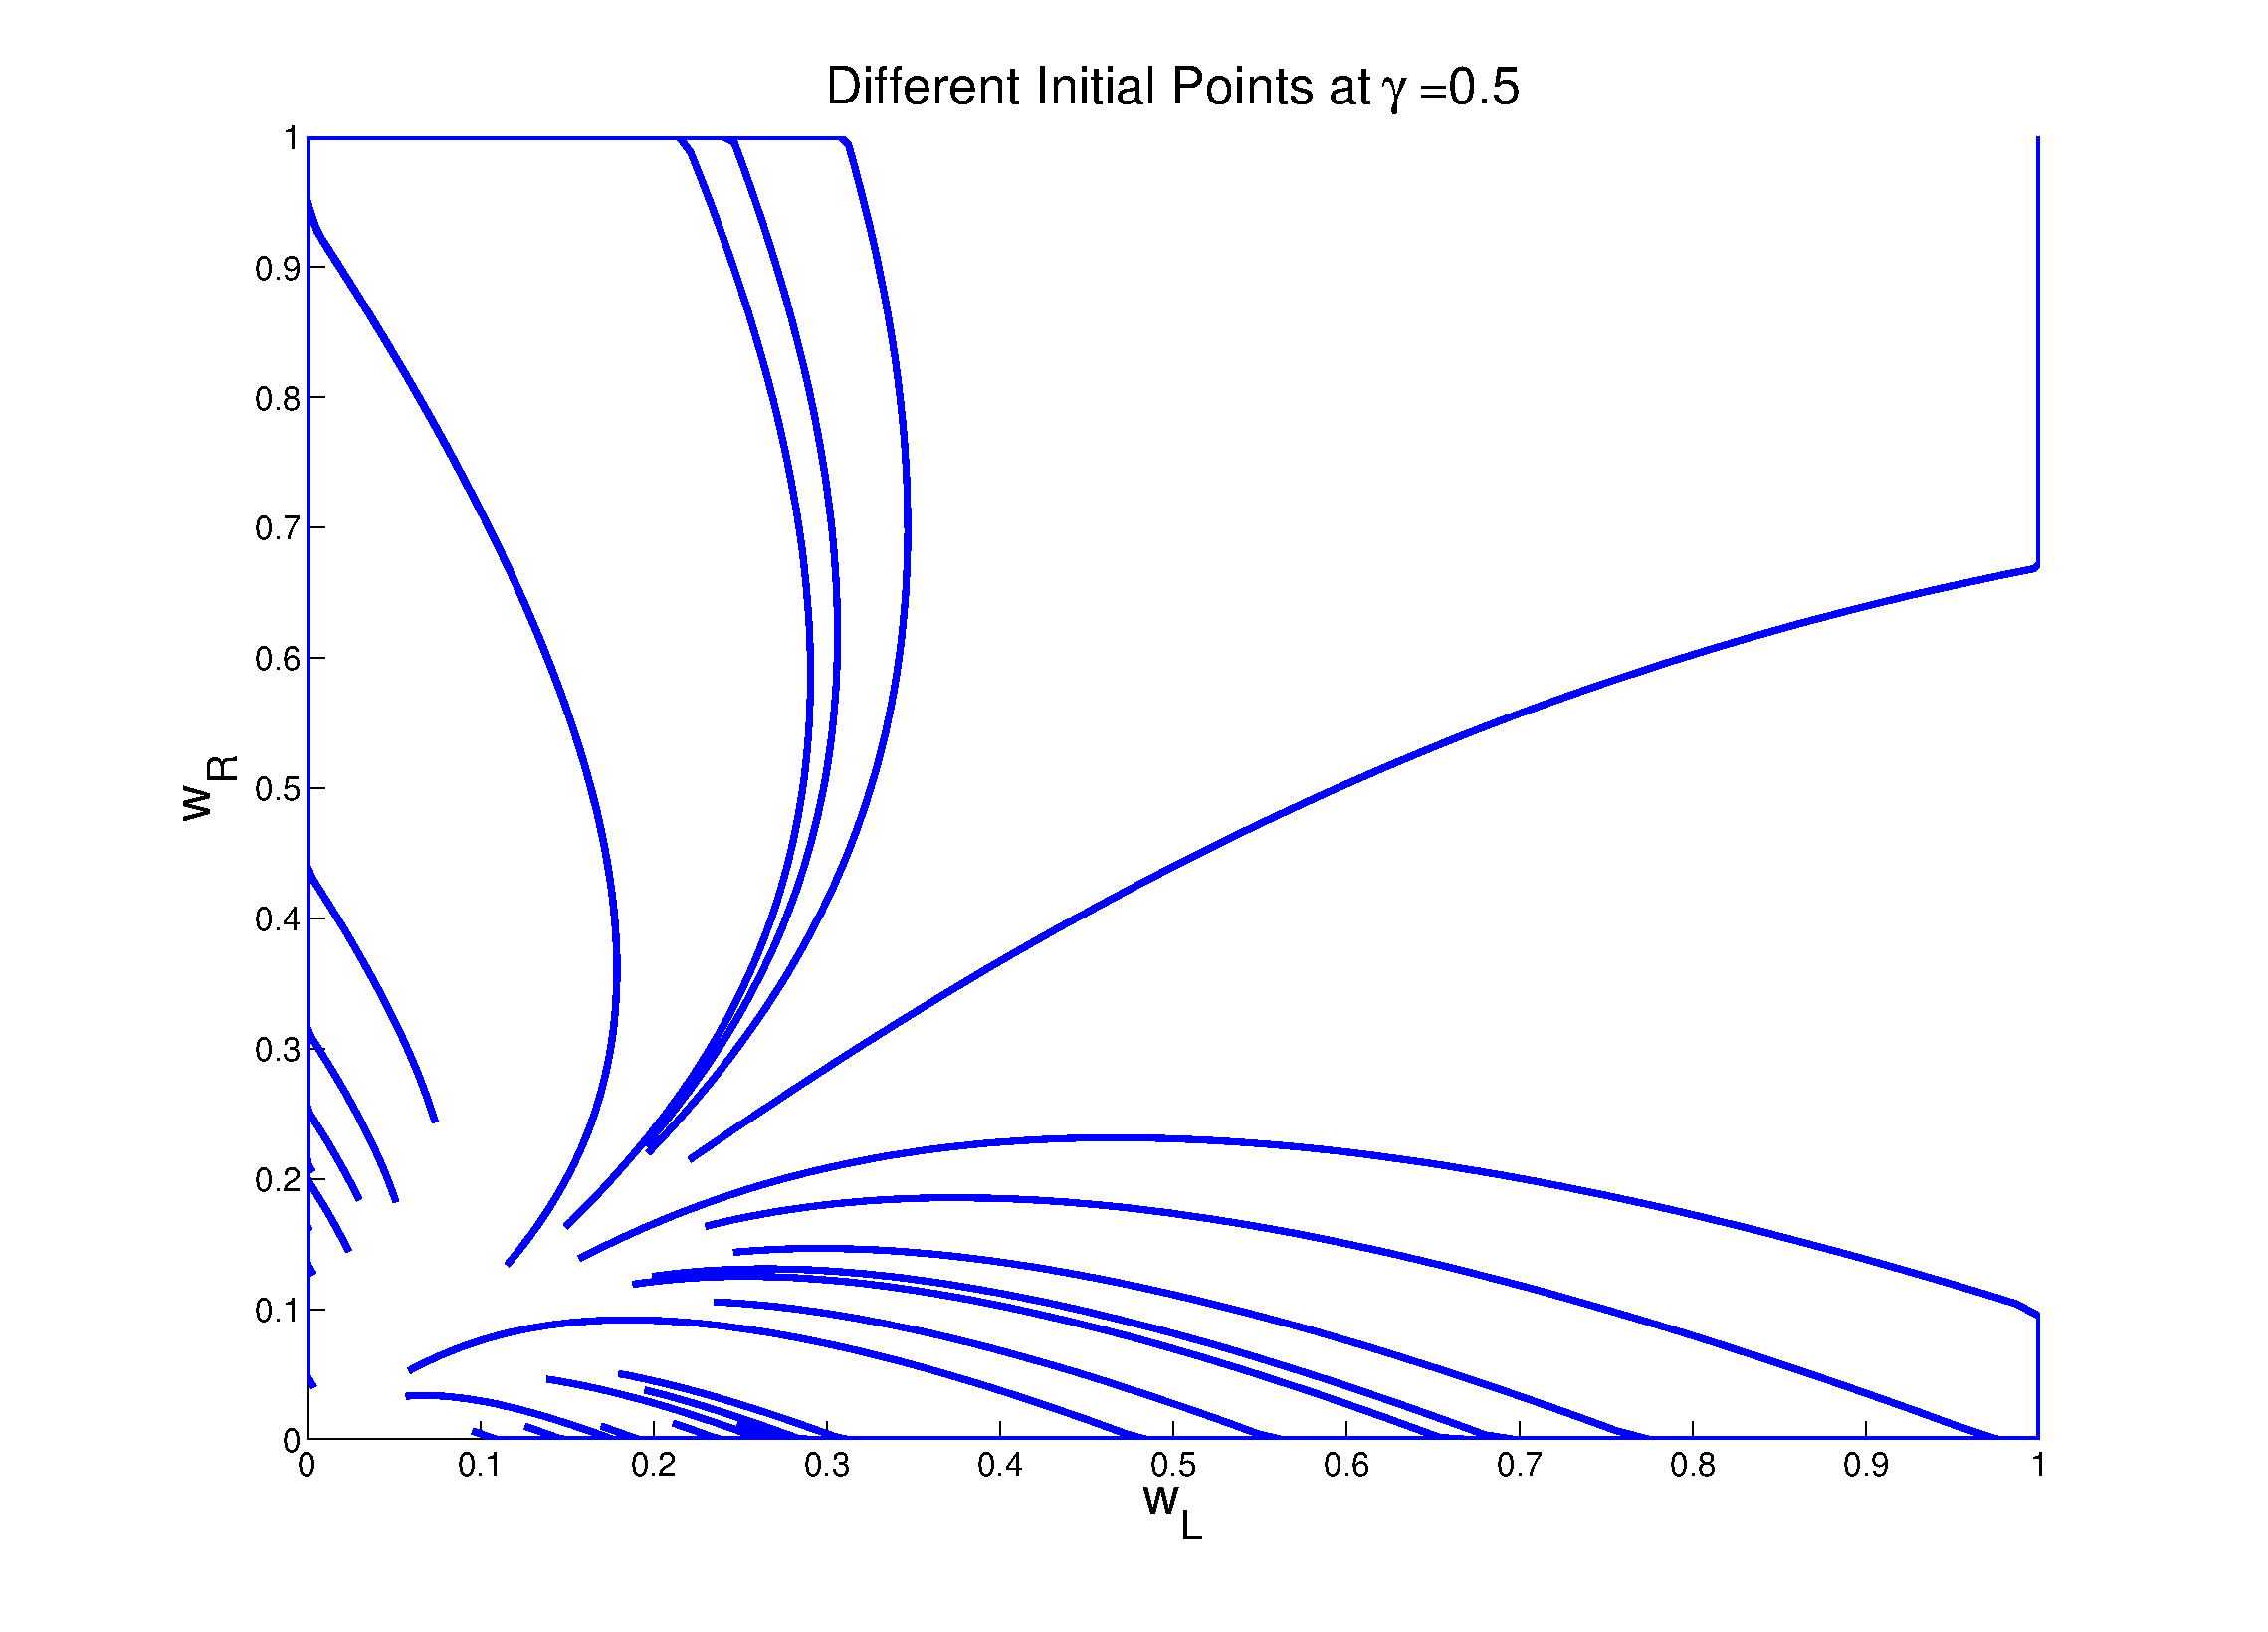
\includegraphics[width=\textwidth]{n_initial.eps}
% tau4_M1.eps: 0x0 pixel, 300dpi, 0.00x0.00 cm, bb= -304   -42   918   834
\begin{footnotesize}
 Figure 8, $\gamma=0.5$ n=30 different initial points randomly chosen between 0 and 0.25 for $w_L$ and $w_R$
\end{footnotesize}
\end{center}

\begin{itemize}
 \item Introduce two further variables, namely, the sum $w_+=w_R+w_L$, and the difference $w_-=w_R-w_L$ of input weights. They can be iteratively calculated as the following: 
\end{itemize}

\begin{equation*}
 \tau_w=\frac{dw_+}{dt}=w_+(c_S+ c_D) \;\;\;\; and \;\;\;\; \tau_w=\frac{dw_L}{dt}=w_-(c_D-c_S)
\end{equation*}

\begin{itemize}
 \item Does the change in initial values mainly concern the combined weight $w_+$ or the difference in weights $w_-$?
\end{itemize}

The provided script from the provided code gives the differences between two of the $w_+$ vectors and $w_L$ vectors:

	\begin{verbatim}
sum(diff(Comp_wplus));     %-5.5511e-017
sum(diff(Comp_wminus));    %9.3782e+014
	\end{verbatim}
The results indicated above with \% signs show that the effect of any change in initial values or $\gamma$ values affects the $w_-$ values more than it does for $w_+$ values. 

\subsection{Discussion}

\begin{itemize}
\item The weights $w_R,w_L$ evolve dynamically in time with the stimulus and then converge into covariance matrix \textbf{C} in this exercise, so called in "unsupervised learning" format. So it is definitely different from the previous "supervised learning" exercise. The purpose is to observe that \textbf{C} converges to monocularity and observe the ocular dominance.

 \item Figure 6 shows that, with increasing $\gamma$ values, the systems go towards the be weighted equally. At the beginning, the neuron gets input from both eyes, then it is tuned under the dynamical effect of covariance matrix. At small $\gamma$ (0,0.25,0.5), the neuron is tuned to the monocularity, at large $\gamma$ (0.75, 1) it tunes to binocularity. Ocular dominance is observed at small $\gamma$ values.

\item Figure 7 indicates the effect of initial value choices for $w_R$ and $w_L$. The ocular dominance is observed as long as both initial values are not equal, otherwise the neuron is tuned to binocularity as in the green line of $w_R(0)=0.15$, $w_L(0)=0.15$. When the $w_R>w_L$, the ocular dominance to the right eye is observed, when $w_L>w_R$ ocular dominance to the left eye is observed.  

\item Figure 8 is another version of Figure 7 added with more initial values. The same discussion also holds here. The probability of being tuned to binocularity seems to be only once in 30 random initial points. 

\item The relation between eigenvectors of \textbf{C} and the evolution of weights: Figure 1-5 show that the blue line dominate mostly for small $\gamma$ values, Figure 6 then shows the fact that, the weights evolve along the principal eigenvector. But, when none of the eigenvectors is dominant, then weights evolve equally towards the binocularity.

\item The change in initial points of the weights concerns mainly $w_-$ rather than $w_+$. This means that, as long as the weights $w_R$ and $w_L$ considerably differ from each other, then their subtraction $w_-$ also get considerably larger than their summation $w_+$. The more the neuron is tuned far from the diagonal green line on Figure 7, the larger the $w_-$ becomes. 

\end{itemize}

\section{One target neuron, with normalization}
The model is now extended with different type of correlations by introducing a normalization.
\begin{equation*}
 v=\textbf{u.w}=w_R u_R + w_L u_L
\end{equation*}
\begin{equation}
 \tau_w=\frac{d\textbf{w}}{dt}=\textbf{Cw}+ \frac{1}{2}\textbf{n.}(\textbf{Cw}) \;\;\;\; with \;\;\;\; 0\leq w_{R,L}\leq 1 \;\;\;\;\;\;\;\; \textbf{n}= \left ( \begin{array}{c} 1 \\ 1 \end{array} \right )
\end{equation}
The differential equation can be solved as the following belove.
\begin{equation*}
 \tau_w \frac{dw_R}{dt}=\frac{1}{2}(c_S w_R + c_D w_L - c_Dw_R - c_Sw_L)
\end{equation*}
\begin{equation*}
 \tau_w \frac{dw_L}{dt}=\frac{1}{2}(-c_S w_R - c_D w_L + c_Dw_R + c_Sw_L)
\end{equation*}

\begin{itemize}
 \item Compute $w_R$ and $w_L$ iteratively as in section 2, use the same $\tau_m$ and $dt$ values as previously, start from initial points of range [0.25, 0.75] for the $w_R(0)$ and $w_L(0)$. Plot $w_L$ versus $w_R$ for different $\gamma$ values and initial points.  
\end{itemize}

\begin{center}
\includegraphics[width=\textwidth, height=80mm]{nomr_gama.eps}
% tau4_M1.eps: 0x0 pixel, 300dpi, 0.00x0.00 cm, bb= -304   -42   918   834
\begin{footnotesize}
 Figure 9, Fixed initial points but different $\gamma$ values
\end{footnotesize}
\end{center}

\begin{center}
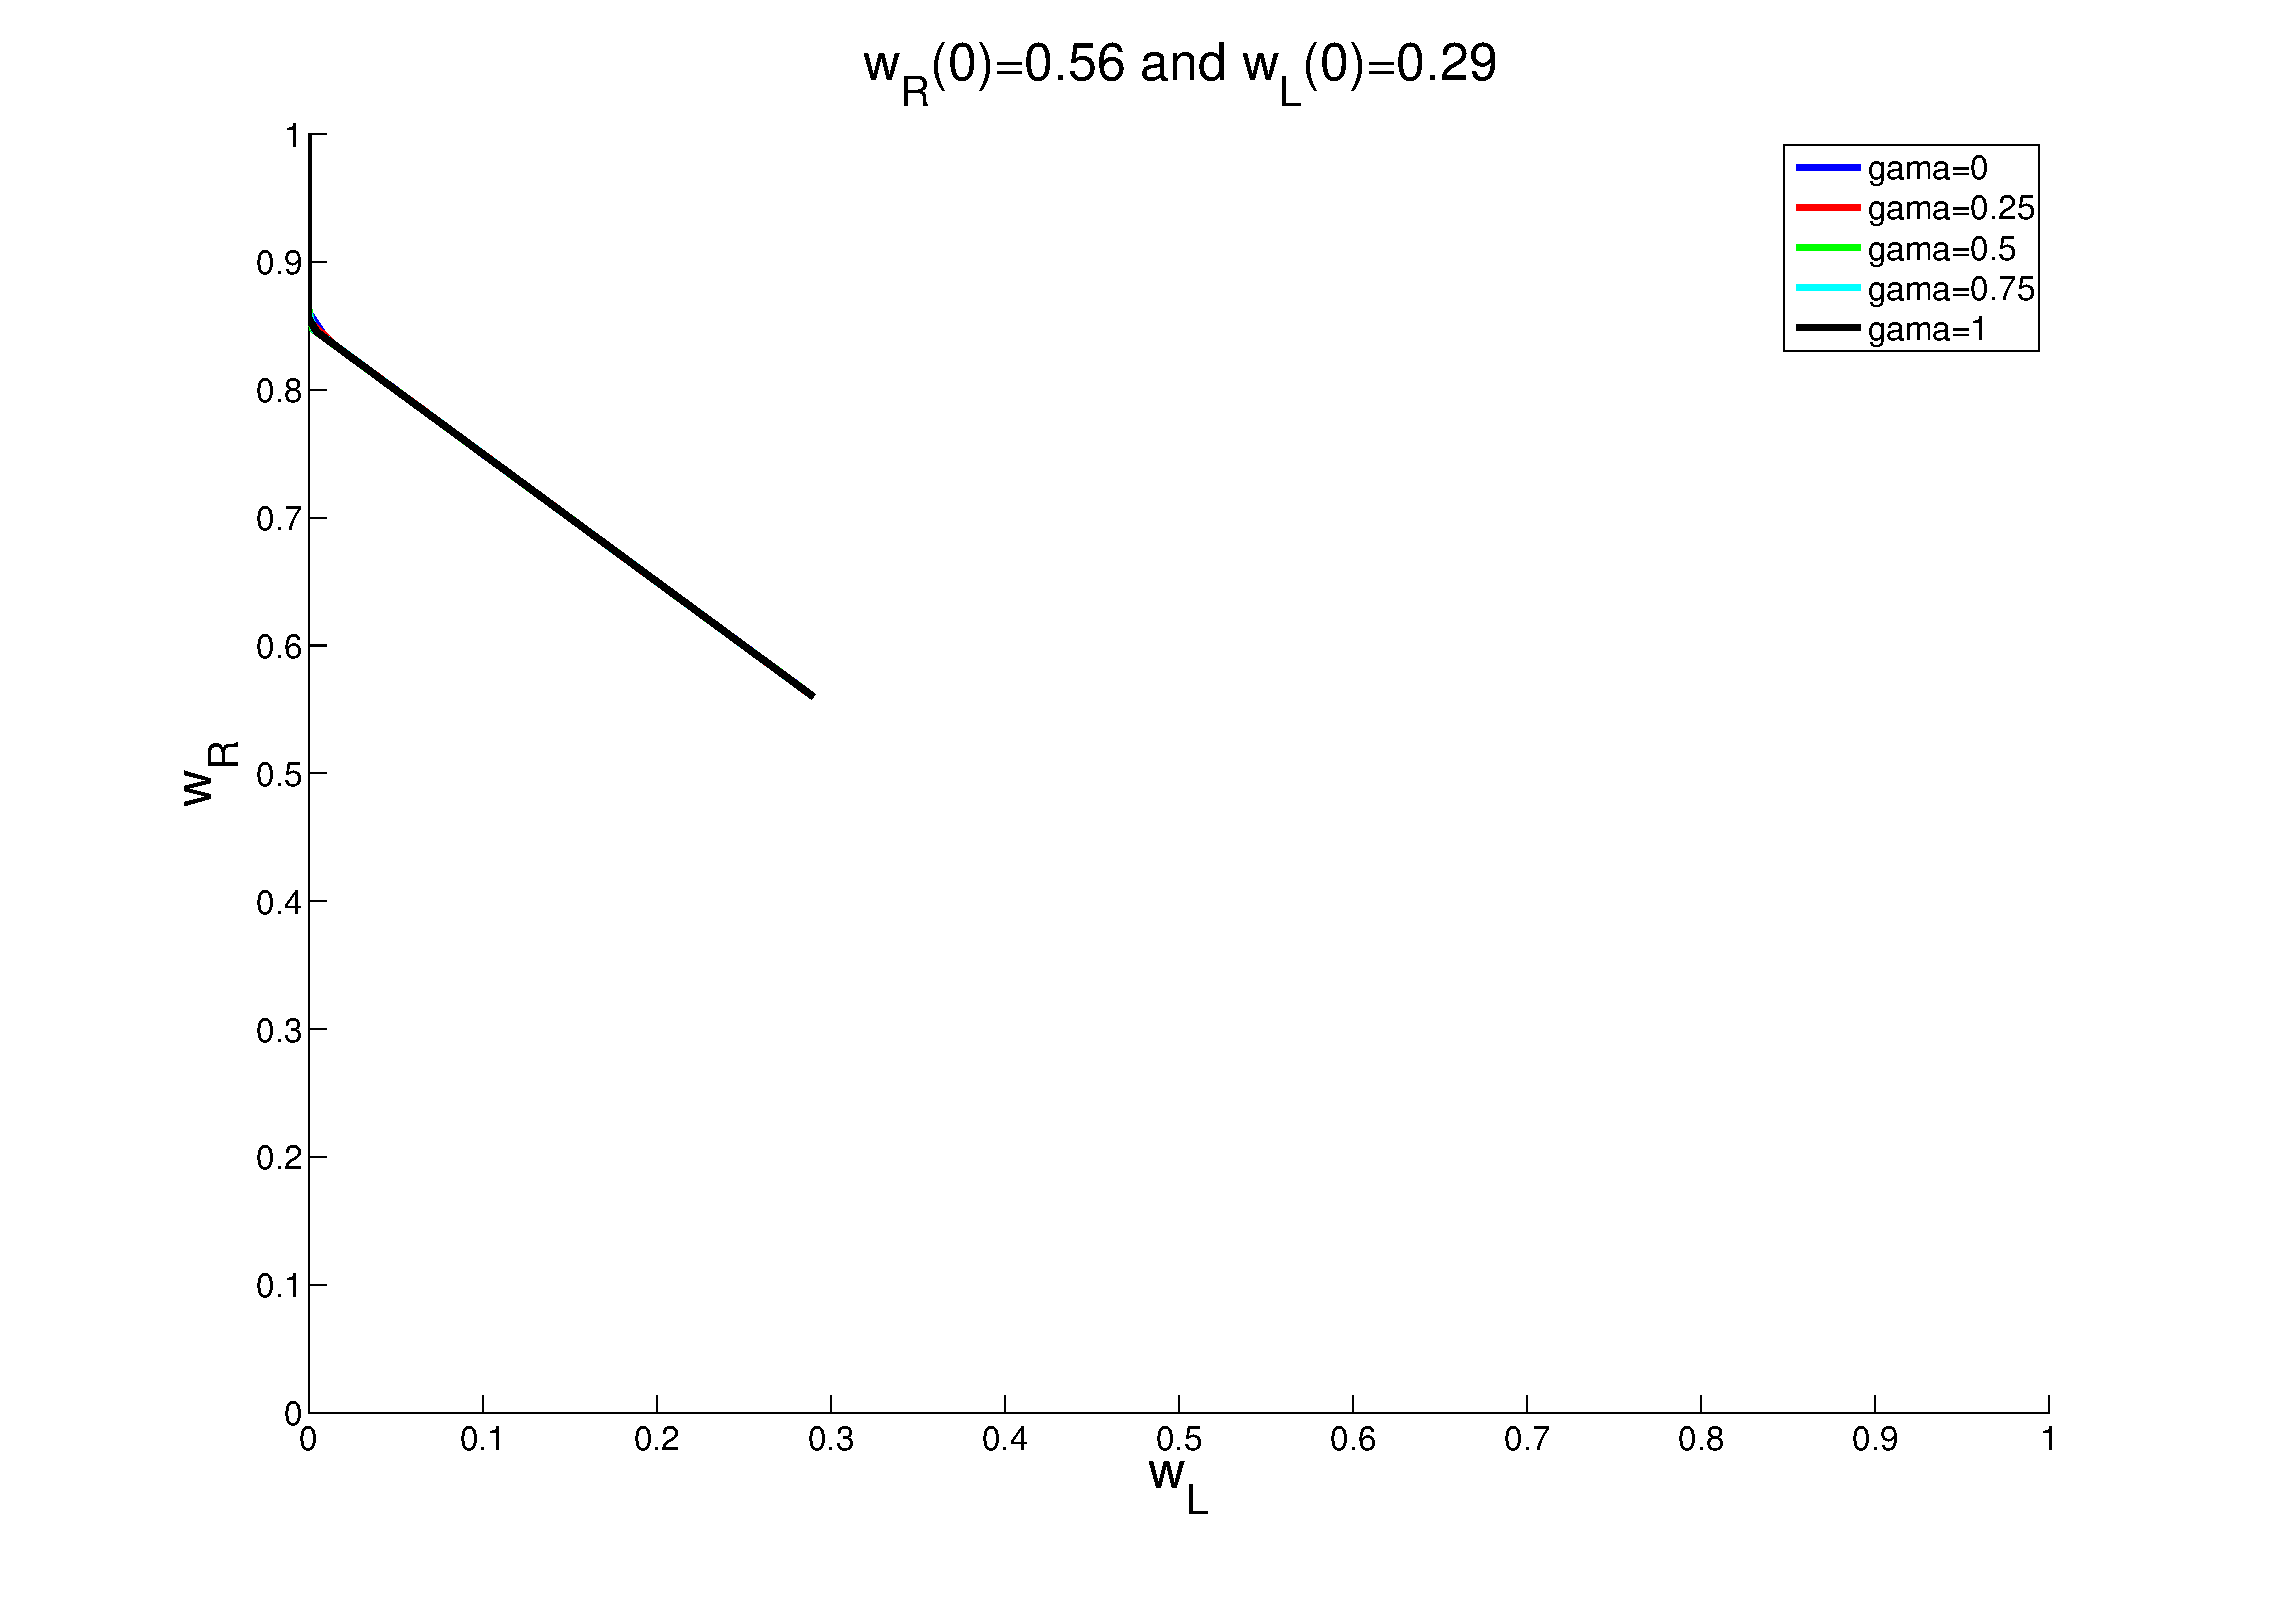
\includegraphics[width=\textwidth, height=80mm]{norm_init.eps}
% tau4_M1.eps: 0x0 pixel, 300dpi, 0.00x0.00 cm, bb= -304   -42   918   834
\begin{footnotesize}
 Figure 10,  Fixed initial points but different $\gamma$ values
\end{footnotesize}
\end{center}

\begin{center}
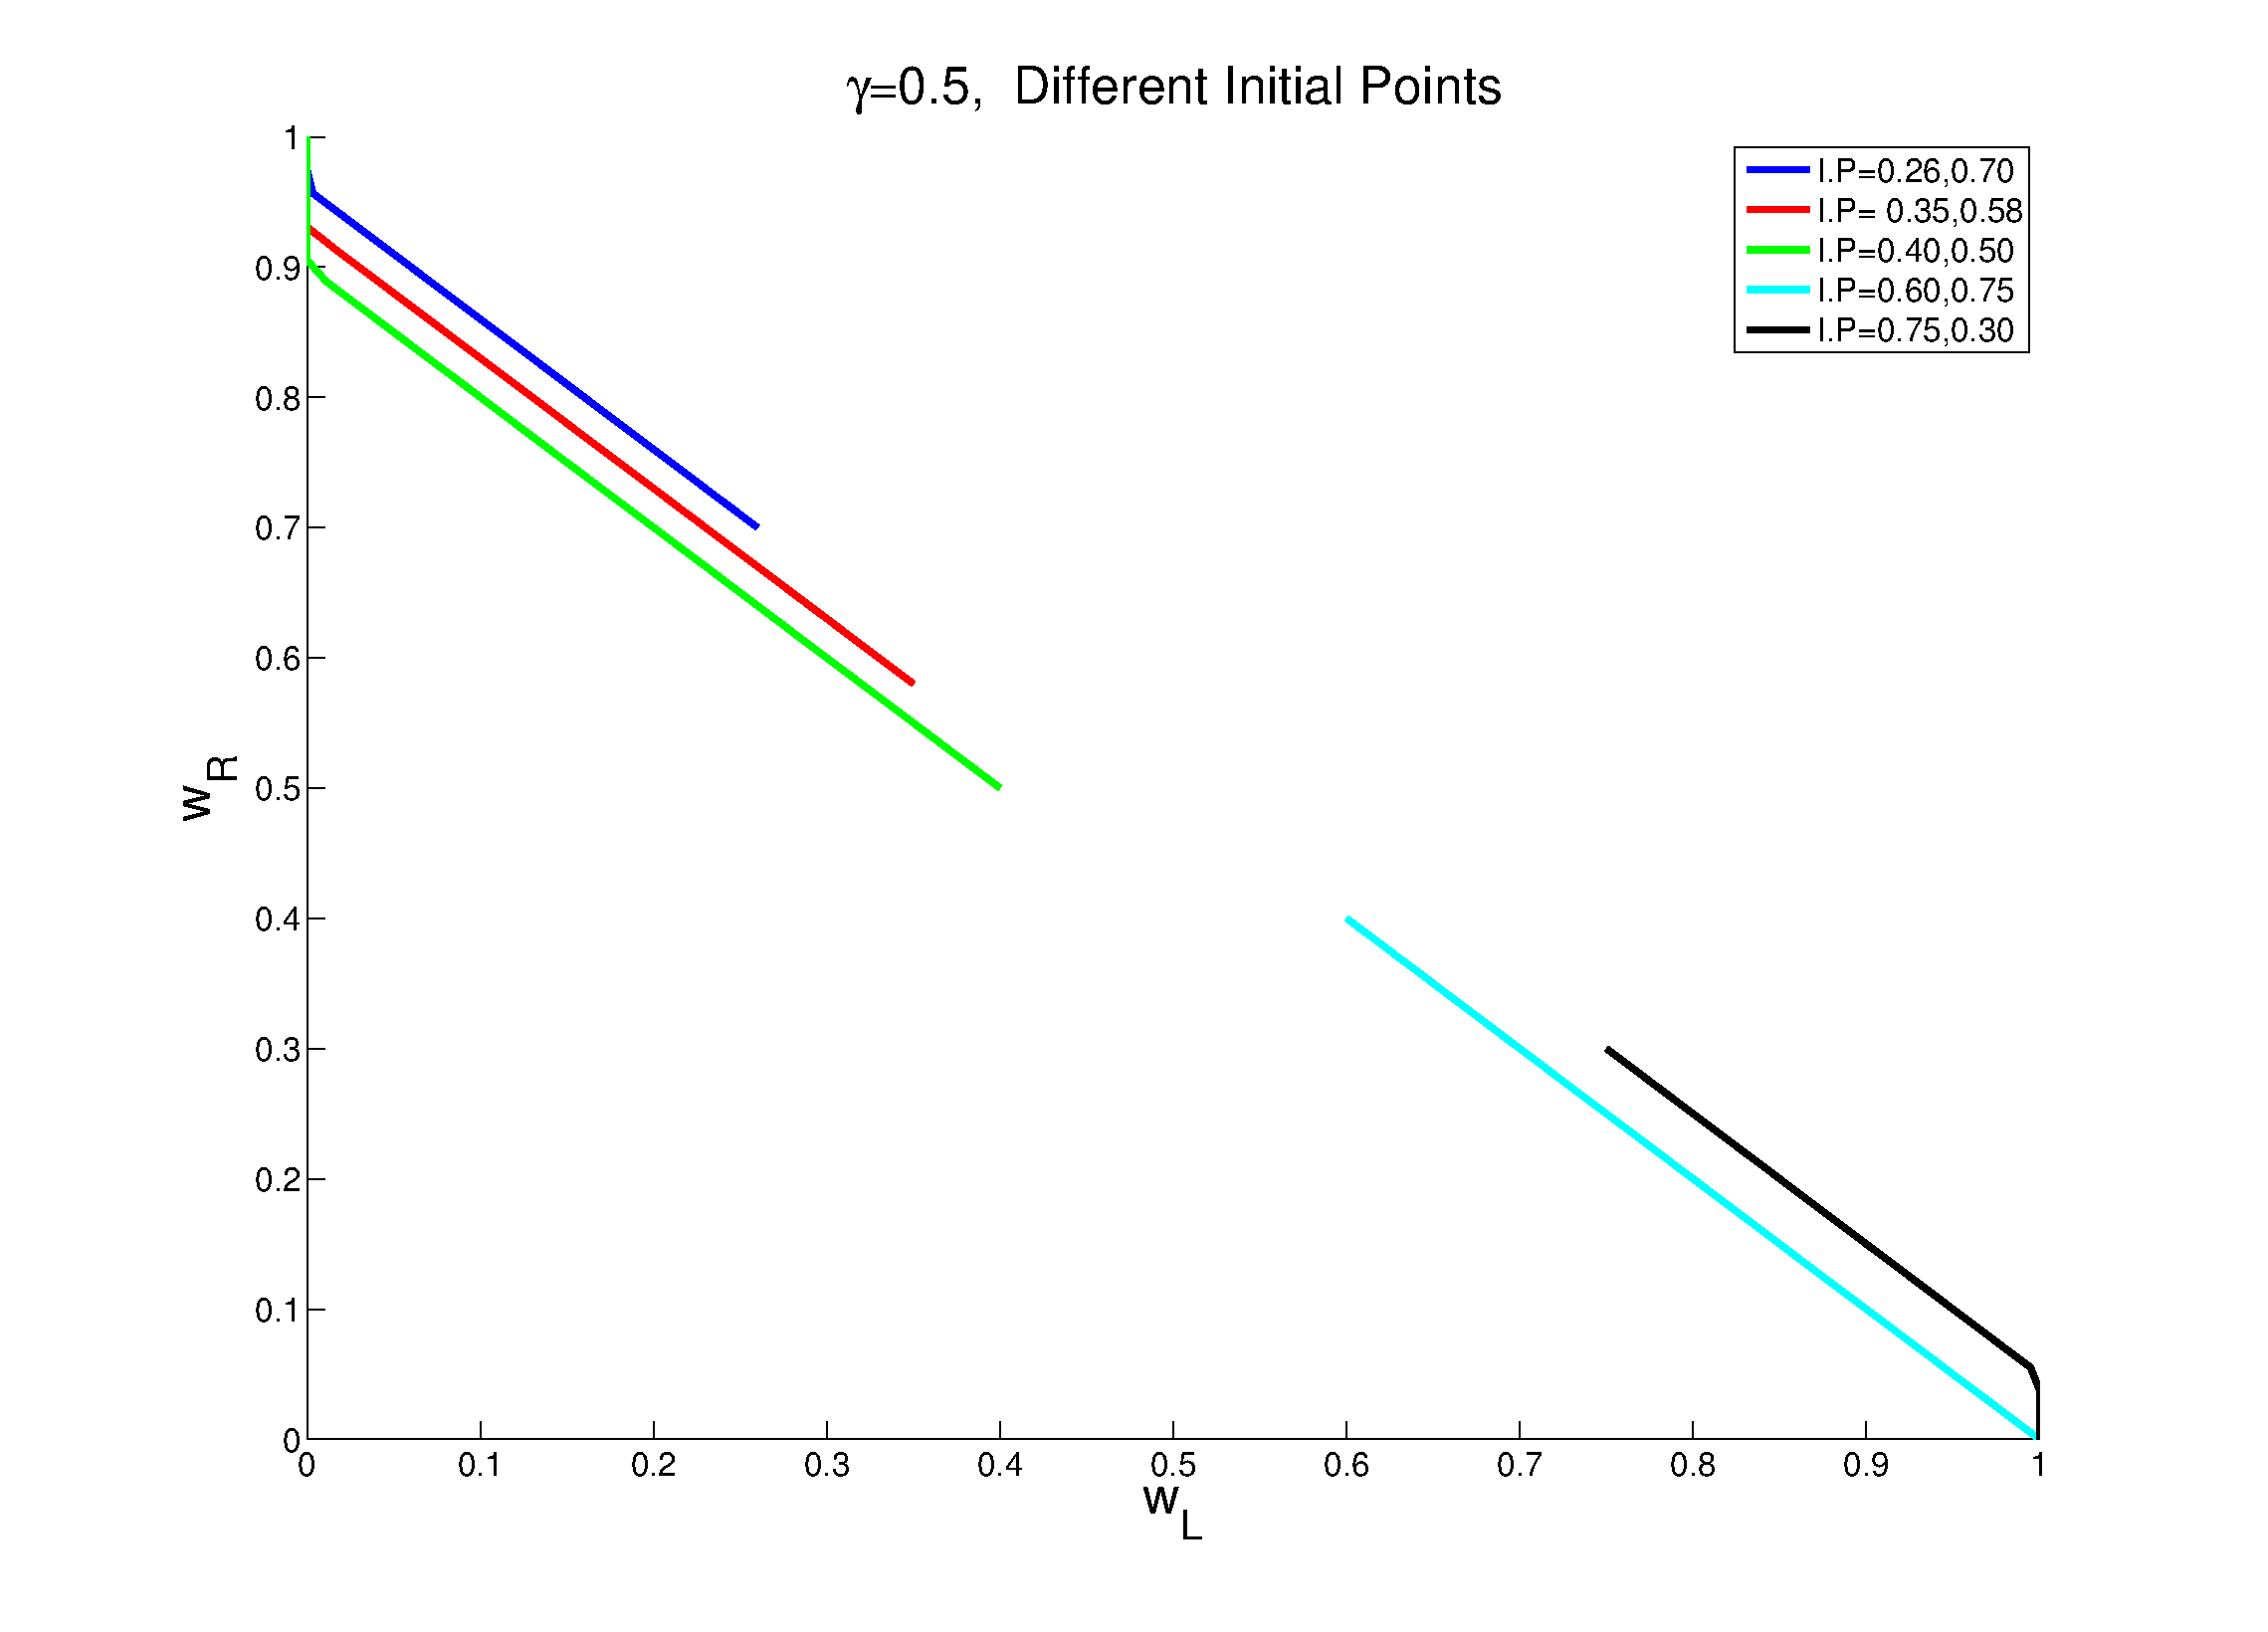
\includegraphics[width=\textwidth]{norm_init1.eps}
% tau4_M1.eps: 0x0 pixel, 300dpi, 0.00x0.00 cm, bb= -304   -42   918   834
\begin{footnotesize}
 Figure 11, $\gamma=0.5$ 5 different initial points (I.P)  $w_L$ and $w_R$
\end{footnotesize}
\end{center}

\begin{center}
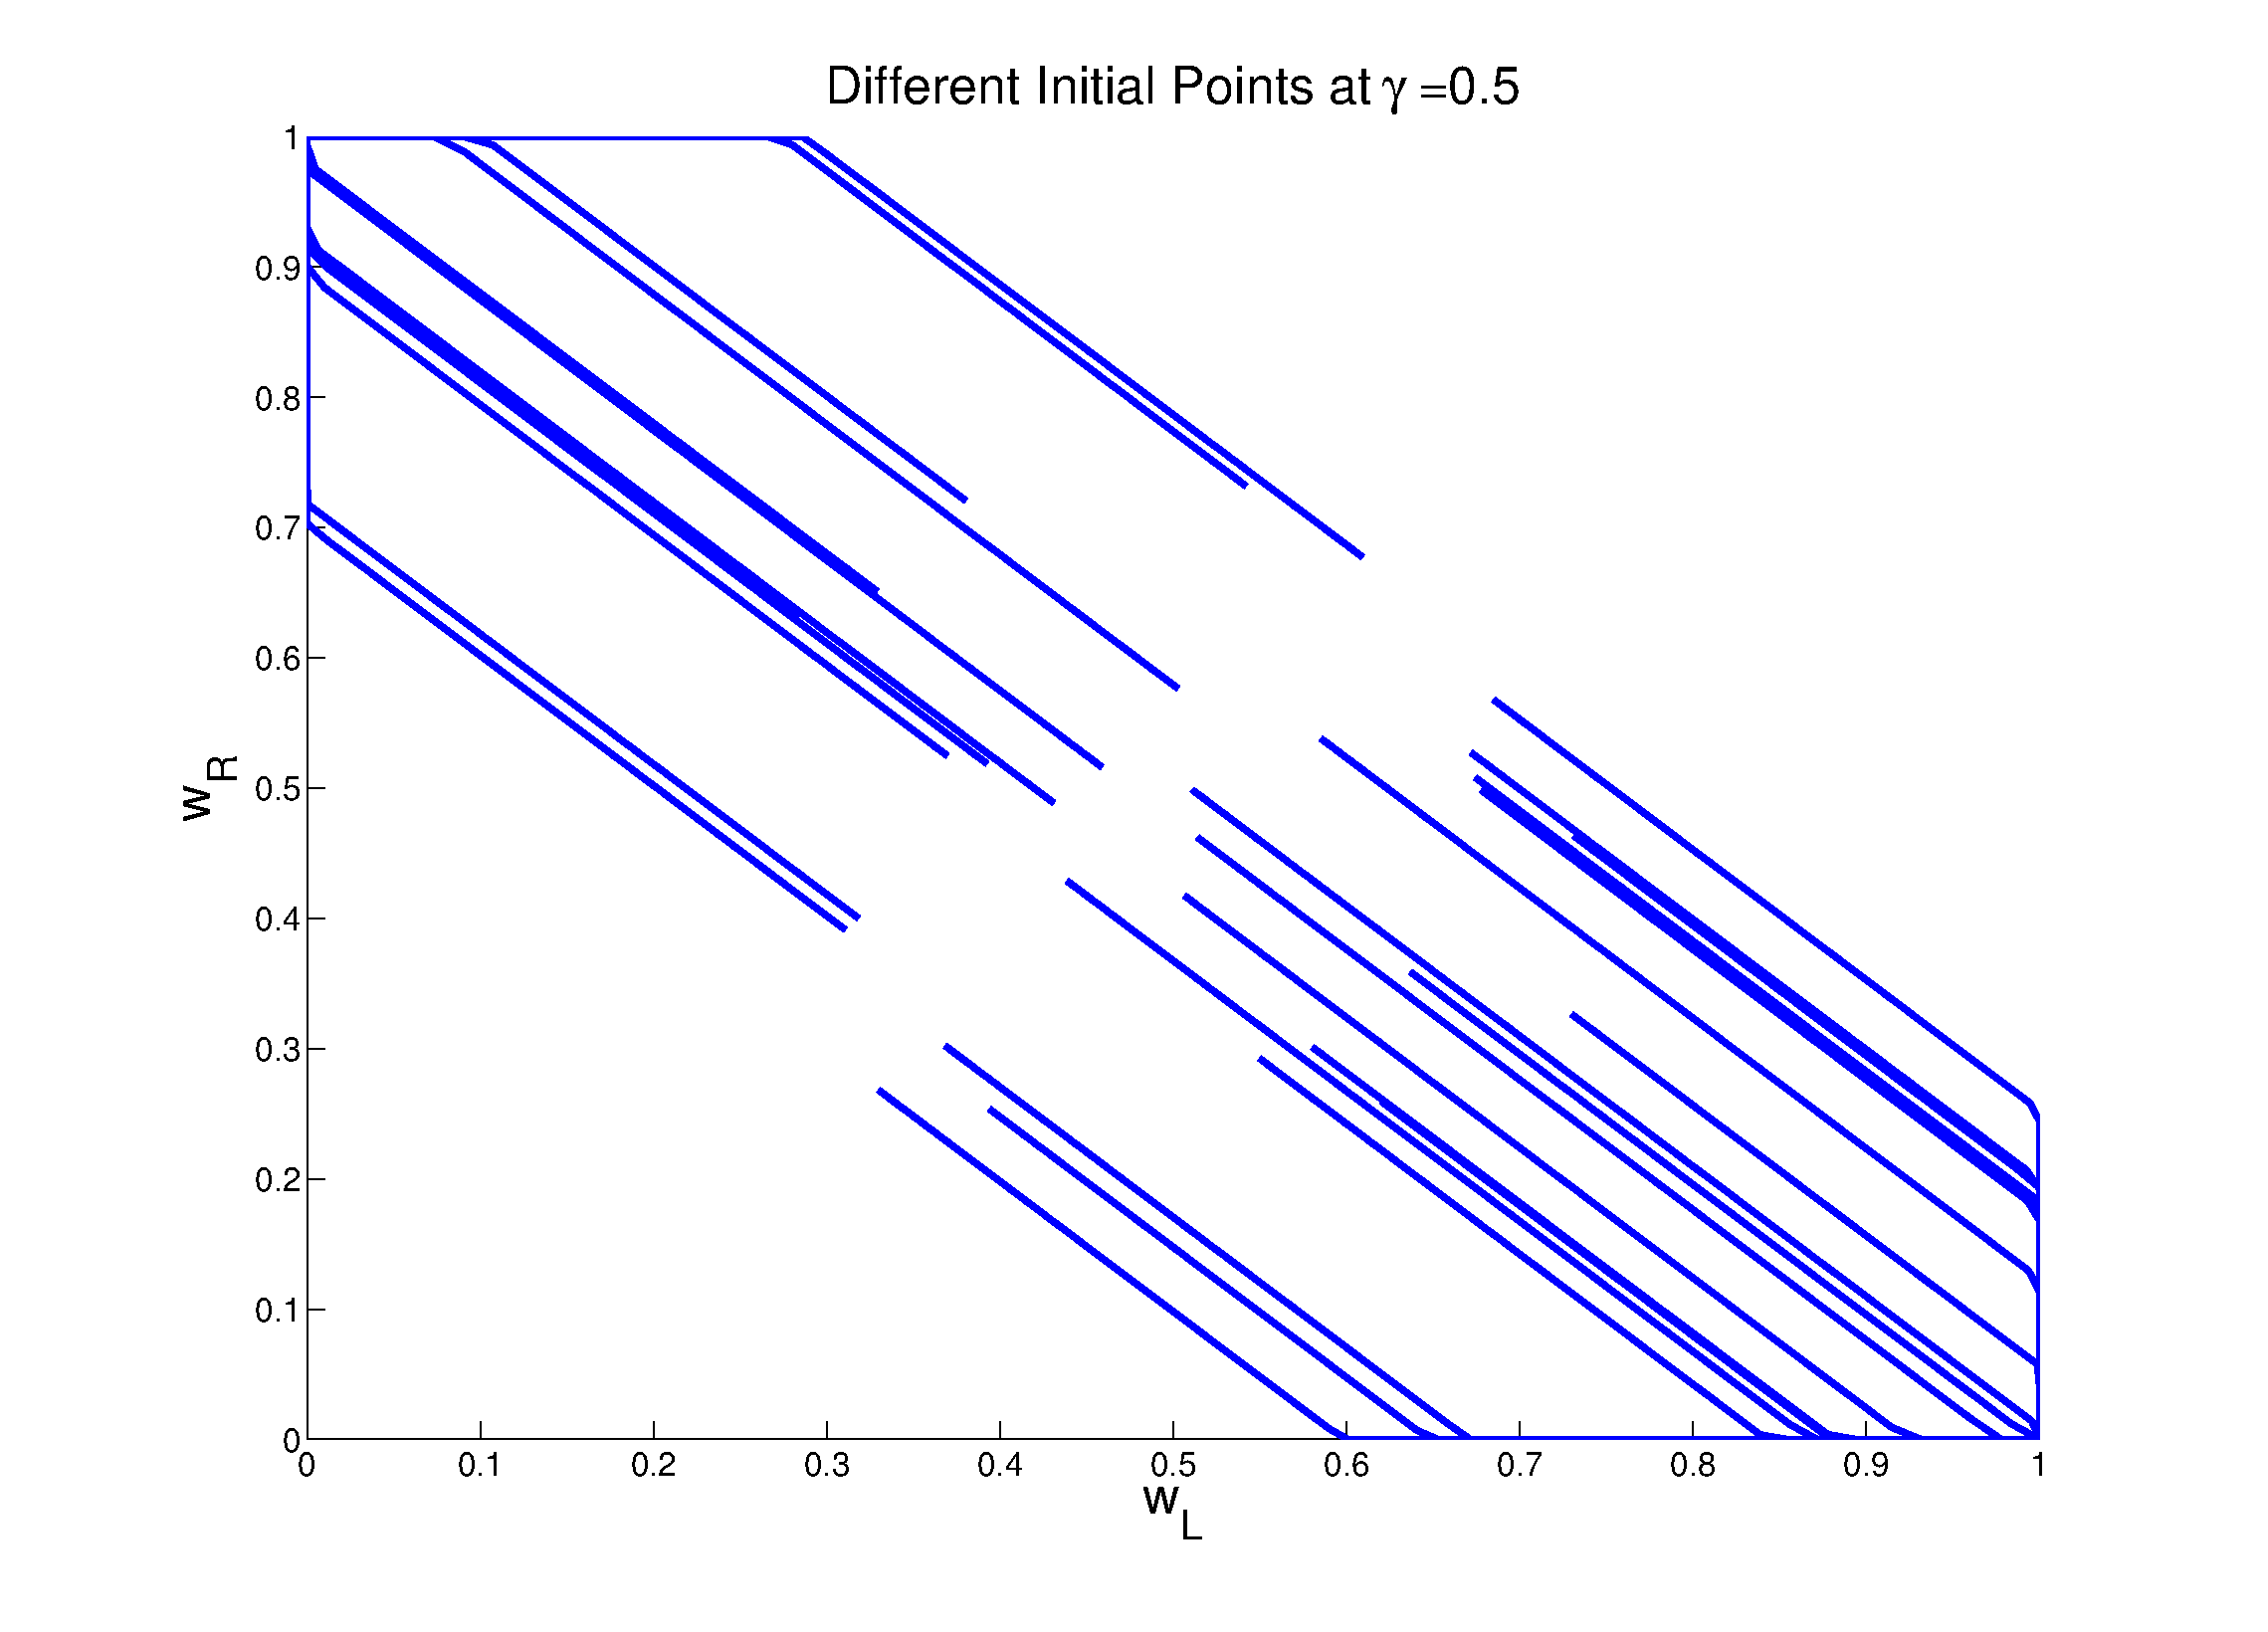
\includegraphics[width=\textwidth]{norm_init2.eps}
% tau4_M1.eps: 0x0 pixel, 300dpi, 0.00x0.00 cm, bb= -304   -42   918   834
\begin{footnotesize}
 Figure 12, $\gamma=0.5$ n=30 different initial points randomly chosen between 0.25 and 0.75 for $w_L$ and $w_R$
\end{footnotesize}
\end{center}

\subsection{Discussion}

\begin{itemize}
 \item There is no observable effect of $\gamma$ for the evolution of $w_R$ and $w_L$ anymore. The neuron is tuned to be monocularity for any $\gamma$ value. If the initial point is closer to $w_L$ as in Figure 9, then the monocularity goes along the left eye, otherwise towards the right eye as in Figure 10.

\item Actually, $\gamma$ directly affects the covariance matrix \textbf{C}, and therefore eigenvalues and eigenvectors. However, as it is already discussed, $\gamma$ does not lead neruon to be tuned to binocularity, the system is now not following the principal eigenvector anymore. Normalization prevents it to grow along principal eigenvector. The growth seems to occur along the second eigenvector. 

\item Different initial value choices in Figure 11 and 12 show that there is always again a sharp monocularity. The binocularity is almost impossible for any initial value choice between 0.25 and 0.75. What matters only for being tuned either towards right or left is initial value choices for the $w_L$ and $w_R$. 

\item When the new $w_+$ and $w_-$ introduced such that
\begin{equation*}
 \tau_m=\frac{dw_+}{dt}=0 \;\;\;\;\;\;\; \frac{dw_-}{dt}=w_-(c_S+c_D)
\end{equation*}
it is expected that $w_+$ is going to have a constant value, and $w_-$ is differ in each iteration. Therefore change in $w_-$ values for different initial values is more likely affectet than $w_+$.

\item The model anaylzed in second part without normalization does not guarantee the monocularity. Thir part with the normalization stabilizes the system to be monocular, and the evolution of weights to be much faster now.

\end{itemize}



\end{document}

